\documentclass[rapport.tex]{subfiles}
\begin{document}
\chapter*{\uppercase{Processus de conception}}
\addcontentsline{toc}{chapter}{PROCESSUS DE CONCEPTION}
\section*{Définition des exigences}
\addcontentsline{toc}{section}{Définition des exigences}
La démarche décrite dans la dernière section permettra de structurer les tâches de conception exécutées par chaque membre de l’équipe. Ainsi qu’avec les informations obtenues dans la revue documentaire, une solution à l’enjeu soulevé en début de projet a été conçue. Les besoins comblés, le fonctionnement de la solution, les différentes solutions explorées et la solution retenue et prototypée seront présentés.
\par
Les responsabilités que la solution développée devra couvrir consistent en : la prise de modèle dans l’environnement réel, la présentation de ces modèles dans l’environnement réel pris par la caméra, la compréhension des coordonnées de l’environnement capturé, la modification du modèle et la reconnaissance des mouvements de l’appareil. La technologie Structure Sensor peut répondre aux responsabilités de prise de modèle dans l’environnement et compréhension des coordonnées de l’environnement réel. Par contre, les autres responsabilités devront être résolues par d’autres moyens.
\par
Deux possibilités se sont révélées comme intéressantes lors des recherches. La première consistant dans le développement d’une solution personnalisée permettant la gestion du modèle déjà scannée. Cette gestion devrait permettre l’ajout du modèle dans un environnement contrôlé à l’aide des coordonnées acquises avec le Structure Sensor. Une fois ajouté dans l’environnement, le modèle doit pouvoir être déplacé, mis à l’échelle et être pivoté. Ce modèle devra pouvoir être supprimé de l’environnement. Toutes ces différentes tâches demandent donc un cadre de développement permettant la transformation des données provenant des périphériques de capture en scène tridimensionnelle avec lesquels les développeurs interagissent.
\par
Un outil répondant à ce besoin a déjà été publié et il consiste dans la deuxième option. Cet outil est la trousse de développement d’Apple, l’ARKit. Celui-ci fait le pont entre les interfaces du périphérique de capture et la trousse de gestion de scène SceneKit. Cette solution est très intéressante puisqu’elle diminue grandement le poids du travail à faire. Par contre, en ajoutant une interface avec une nouvelle frontière, on ajoute aussi des contraintes au développement. De plus, l’ARKit permettant son usage avec des appareils n’ayant pas de Structure Sensor représente des possibilités fonctionnelles plus limitées. Un exemple de ces limitations est la détection d’objet en premier plan de la scène. Autrement dit, cacher un modèle numérique par un objet réel en le plaçant dans le monde réel est malheureusement impossible.
\par
Afin de diminuer la grosseur du travail à faire, la solution de l’ARKit a été sélectionnée. Les limites que celle-ci importe ne seront pas atteintes dans le contexte du projet. Toutefois, une poursuite de projet pourrait atteindre ces limites.
\par
\begin{longtable}{|c|p{4.5cm}|p{10cm}|}\hline%
    ID & Titre & Description \\\hline\hline
    \csvreader[late after line=\\\hline,
    table head=\caption{Liste des exigences}\label{tab:exigencesPlanif}\\\hline]
    {./exigences.csv}{id=\id,titre=\titre,description=\description}%
    {\id & \titre & \description}
    \caption{Liste des exigences}
\end{longtable}
\section*{Risques et hypothèses}
\addcontentsline{toc}{section}{Risques et Hypothèses}
Dans un projet de cette envergure, les risques sont nombreux et importants. Afin d’assurer une bonne planification et une bonne gestion de ceux-ci, une réunion a été convoquée pour identifier ces risques et élaborer une stratégie de mitigation dans le but d’atténuer leurs impacts. La liste ci-dessous présente les différents risques qui ont été ciblés avec leur cote d’impact et de probabilité ainsi qu’un résumé de la stratégie de mitigation prévue.
\begin{longtable}{|p{3.5cm}|p{2.75cm}|p{2.75cm}|p{6cm}|}\hline%
    Risque & Impact & Probabilité & Migration é atténuation \\\hline\hline
    Les difficultés d’implémentation des interfaces de programmation peuvent bloquer le développement. & Très important & Très probable & Afin de réduire l’impact de ce risque, les attentes du produit final ont été réduites afin de laisser assez liberté à la résolution de problème. De plus, des rôles ont été assignés à des membres de l’équipe en fonction des interfaces de programmation ce qui permet le travail de chacun en parallèle. \\\hline
    La dépendance à une technologie matérielle, le Structure Sensor, peut amener une réduction dans le temps de développement. & Très important & Très probable & Afin de limiter cette dépendance, l’équipe a décidé de manipuler les modèles 3D à l’aide de la trousse de réalité augmentée Apple. Les développeurs ayant chacun accès à un appareil Apple certains pourront se concentrer sur l'ARKit sans avoir besoin du senseur. \\\hline
    Les tests automatisés d’interface mobile sont complexes à implémenter. & Important & Probable & Des tests unitaires seront développés pour toutes les fonctions qui ne sont pas directement en contrôle de l’interface graphique. Les responsabilités du code côté interface seront limitées et feront principalement appel à des fonctions tests de façon unitaire. \\\hline
    Il y a un manque de documentation pour le Structure Sensor ce qui peut limiter la vitesse de développement. & Important & Probable & Une validation des ressources disponibles a été faite préalablement à la validation de la sélection du projet. La documentation officielle est en effet dommage, toutefois le nombre d’exemples disponible et la présence d’un forum de développeur laissent croire que les problèmes seront résolus. \\\hline
    Il n’y a pas de propriétaire du produit ou client officiel, la vision du produit final peut donc être perdue au cours du développement. & Peu important & Peu probable & Lors de la première rencontre d’équipe, chacun des membres à identifier ces attentes par rapport au produit final. Un résumé de la vision de chacun et une synthèse de la solution attendue ont été pris en note. \\\hline
    \caption{Liste des risques}
    \label{risquesPlanif}
\end{longtable}
\par
En plus des risques (présenté ci-haut), une liste d’hypothèses a aussi été produite dans le but de prédire et de prévoir l’impact de certains éléments sur le projet. Celle-ci est présentée ci-dessous et contient la catégorie ainsi que l’auteur de cette hypothèse.
\begin{longtable}{|c|p{4.5cm}|p{10cm}|}\hline%
    ID & Titre & Description \\\hline\hline
    \csvreader[late after line=\\\hline,
    table head=\caption{Liste des hypothèses}\label{tab:hypPlanif}\\\hline]
    {./hyps.csv}{id=\id,titre=\titre,desc=\desc}%
    {\id & \titre & \desc}
    \caption{Liste des hypothèses}
\end{longtable}
\section*{Avancement itératif}
\addcontentsline{toc}{section}{Avancement itératif}
\subsection*{Itération 0}
\addcontentsline{toc}{subsection}{Itération 0}
\subsubsection*{Conception}
\addcontentsline{toc}{subsubsection}{Conception}
\paragraph*{Composantes à intégrer}
\addcontentsline{toc}{paragraph}{Composante à intégrer}
Un travail préliminaire à la réalisation du travail fu de lister les différentes composantes qui devaient être intégrer dans notre application. Cette liste permet au développeur de comprendre l'envergure du travail à accomplir. De plus, elle permet une compréhension simple de chaque partie du projet même, si on n'a pas travaillé dessus.
\begin{figure}[H]
    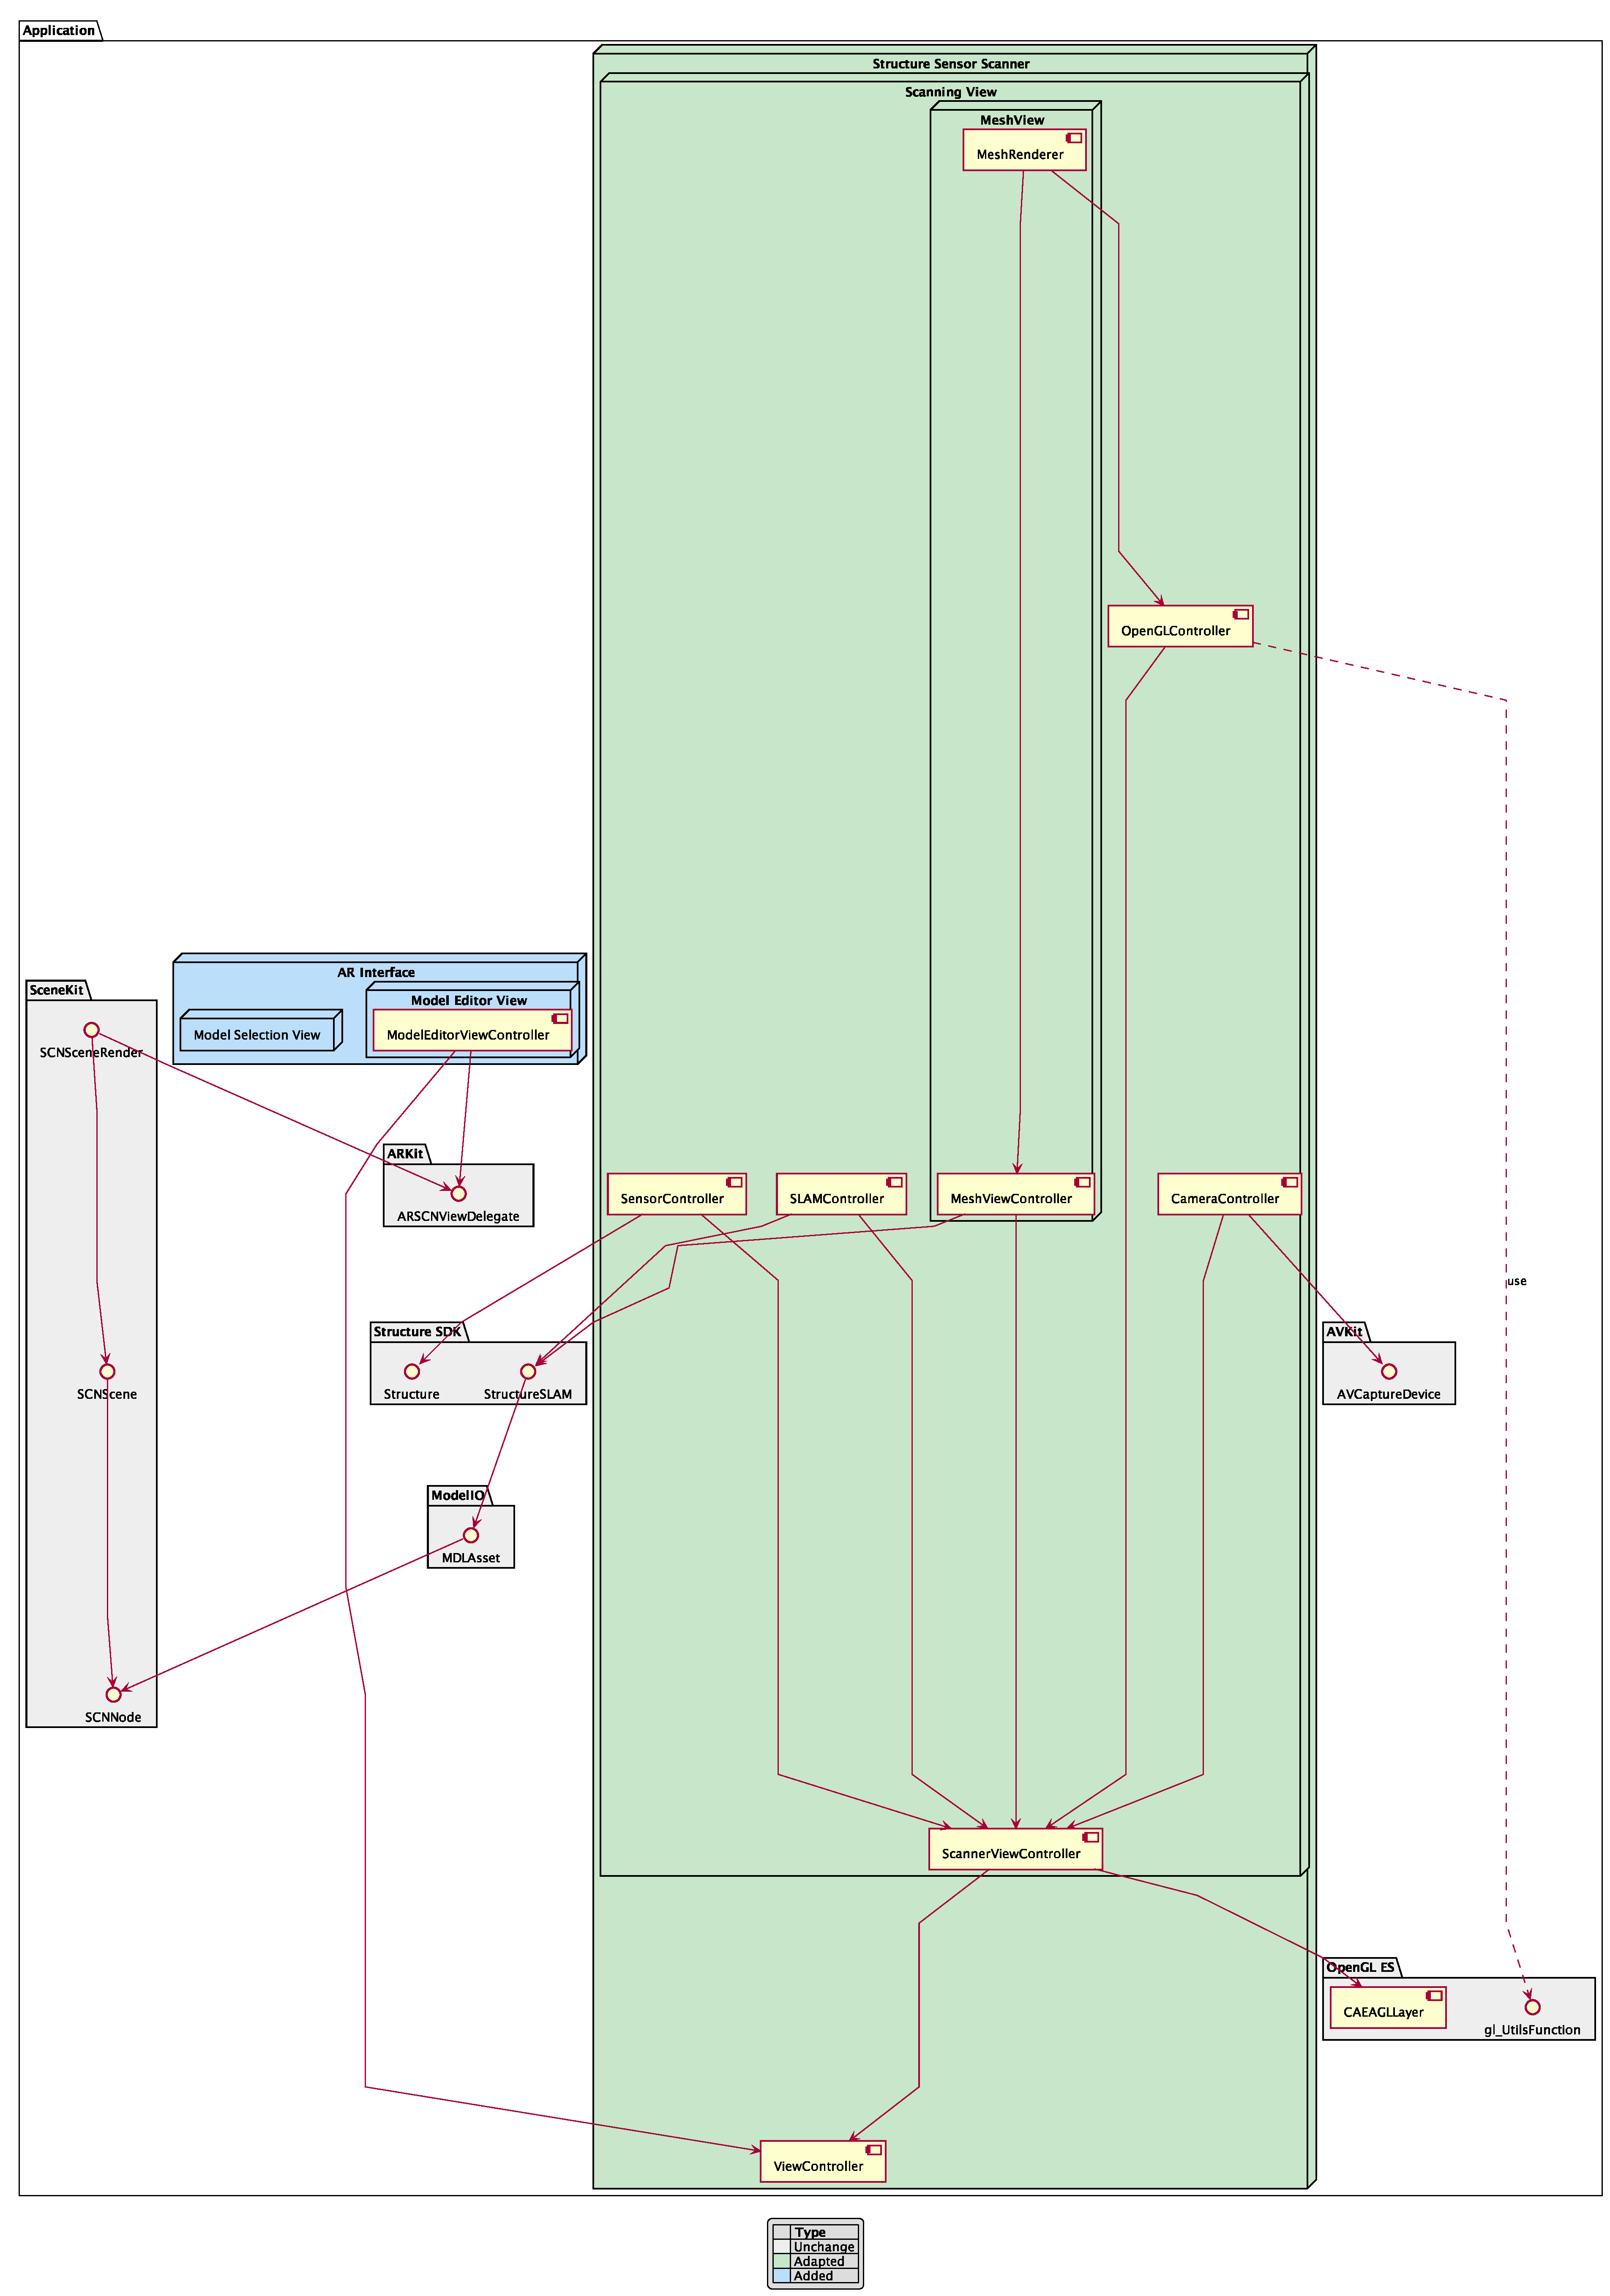
\includegraphics[width=0.5\textwidth]{project-architecture.eps}
\centering
    \caption{Diagramme des composantes de l'application}
\end{figure}
\par
Comme on peut le voir, le produit, lorsqu’implémenter avec l’ARKit, consiste en une application intégrant plusieurs interfaces. Ce qui représente définitivement un aspect facilitant au développement. Toutefois, un tel choix présente des limites et demande une adaptation de l’application pour réduire la friction aux frontières de chacune.
\par
Les différentes interfaces font face à une variété d’enjeux et intègre une variété de technologies produite non seulement par Apple. L’interface de réalité augmentée récemment développée par Apple, ARKit. Cette librairie a pour principale tâche, l’intégration des fonctionnalités de la caméra et de la détection de mouvement afin de créer une expérience de réalité augmentée.\citep*{aRKitDoc}
\par
Cette API est utilisée en coopération avec le SceneKit l’interface de gestion d’environnement 3D dans iOS aussi produit par Apple. Celle-ci simplifie les principaux défis du développement 3D comme les animations, la simulation physique, les effets de particules et le rendu réaliste avec gestion d’effet de lumière. L’usage d’une interface produite par le propriétaire de l’appareil hôte de l’application permet de s’assurer d’une optimisation fournie.\citep*{sceneKitDoc}
\par
Les modèles utilisés par les scènes proviennent de modèle 3D importé par l’interface de Model I/O, ils sont convertis par la suite en ScnNode. Le modèle permet la gestion des textures, des fichiers, des caméras et des matériaux.\citep*{modelIODoc} Ce genre de modèle n’est pas propriétaire à Apple, il peut donc être utilisé par Unity\citep*{unityDoc} et Blender\citep*{blenderForumsRichardMarklew}.
L’importation des modèles 3D se fait à l’aide du senseur Structure qui est une des principales technologies du projet. Ce périphérique utilise la caméra de la tablette et la caméra sur le périphérique pour avoir une meilleure compréhension de l’environnement 3D. Le périphérique contient aussi un senseur infrarouge pour faciliter l’interprétation de l’environnement. Un kit de développement logiciel est fourni par les développeurs du périphérique permettant le contrôle du senseur et l’exportation en modèle.\citep{occipitalsdk} Les images capturées par le senseur et la caméra sont par la suite présentées par l’interface de programmation AVKit. La classe AVCaptureDevice est ainsi utilisée pour présenter à l’usager l’environnement pris par l’appareil.\citep*{aVKitDoc} Afin d’offrir un rendu plus réaliste, la librairie OpenGL est aussi utilisée.\citep*{openGLESDoc}
\par
Les liens entre la logique de notre application et celle des API se font par des extensions aux contrôleurs des vues principales de notre application et par l’intégration de certaines interfaces. Les interfaces de Structure, OpenGL, AVCaptureDevice se font par l’extension du contrôleur de vue du scanneur. Pour ce qui est de l’ARKit et SceneKit, les classes respectant le patron « delegates » pour chacun ont été implémentées dans le contrôleur de la vue de manipulation de modèle.
\par
Chacun des contrôleurs est lié à une vue dans le storyboard et par les liens créer par la logique ou par ceux créer dans le storyboard, ce qui permet à l’usager de transférer d’une à l’autre.
\subsubsection*{Réalisation}
\addcontentsline{toc}{subsubsection}{Réalisation}
Dans la méthodologie AGILE, les projets se doivent de commencer avec une itération 0. Le but de cette itération est de devoir élaborer les spécifications et la portée du projet avec le client. Cette itération a débuté avec une rencontre avec monsieur Carlos Vasquez afin de savoir ce qui serait inclus dans cette session de développement. Ce qui est sorti de ses rencontres avec le client et avec les coéquipiers de l’équipe était la liste des exigences présentée précédemment et un calendrier des itérations. Carlos semblait ravi de l’idée de faire plusieurs points de contrôle avec lui tout au long de la session afin de rectifier le tir sur le travail accompli et restant à accomplir.
\newpage
\subsection*{Itération 1}
\addcontentsline{toc}{subsection}{Itération 1}
\subsubsection*{Conception}
\addcontentsline{toc}{subsubsection}{Conception}
\begin{figure}[H]
    \includegraphics[width=\textwidth]{DSS_AjoutModels.png}
\centering
    \caption{Diagramme de séquence d'ajout d'un modèle}
\end{figure}
Dans le diagramme ci-haut, on peut voir l'interaction entre les classes afin de pouvoir ajouter un modèle dans une scène de réalité augmentée. Quand un utilisateur clique sur l’écran, l’action est détectée par le storyboard. Un storyboard est la classe qui gère les composantes visuelles d’une application IOS. Il y a plusieurs types de gestes pouvant être détectés par le storyboard, mais pour ce scénario, seulement le simple toucher est détecté. Une fois détecté, le storyboard envoie le type de geste au contrôleur de la vue. Ici ce contrôleur reçoit un geste de type “UITapGesture” et la méthode “UITapGestureRecognizer(point)” est appelée. L’argument point de la méthode possède plusieurs informations sur le geste, dont les coordonnées spatiales, pour savoir où déposer le modèle. Dans cette méthode, il y a un appel à la classe “SCNScene” qui possède une méthode afin de savoir si le point est dans la zone de surface détecté auparavant. Si c’est le cas, on ajoute le modèle à la scène virtuel, ce qu’y va générer la vue avec le nouveau modèle à la position souhaité. Pour être détecté comme un simple touché, il y a une limite de 0.3 seconde, sinon le geste est un long touché ce qu’y résulte en un autre type de geste qui sera traité plus tard.
\newpage
\paragraph*{Scan}
\addcontentsline{toc}{paragraph}{Scan}
Lors de la première itération, le processus de conception du module de scan a aussi débuté. La procédure suivante devra être implémentée pour permettre un scan avec le Structure Sensor.
\begin{figure}[H]
    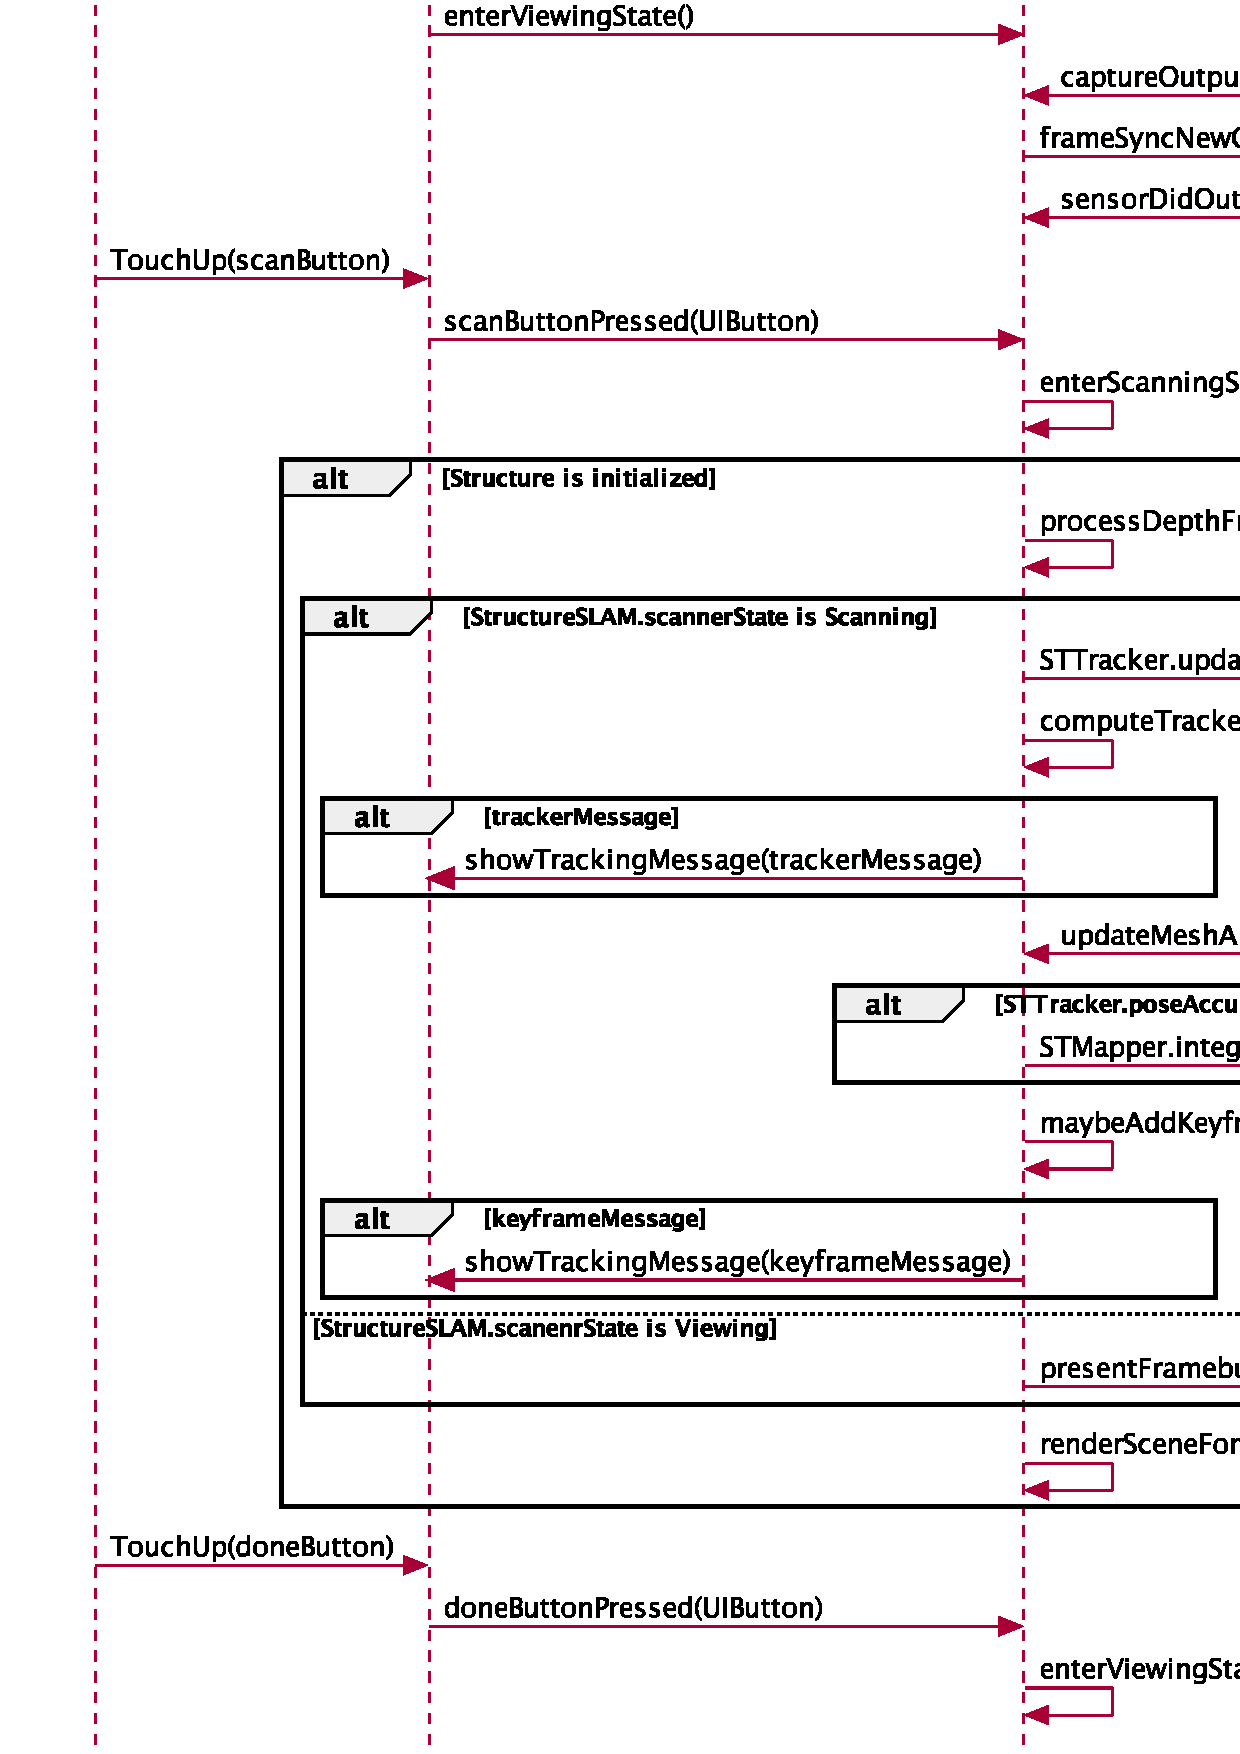
\includegraphics[width=\textwidth]{diagrams/dss-scanner.png}
\centering
    \caption{Diagramme de séquence d'un scan d'objet}
\end{figure}
Le diagramme de séquences pour le scan d’un modèle montre les étapes nécessaires à produire un modèle d’objet scanner. Les premières étapes avant la première interaction avec l’usager sont effectuées au lancement de l’application. Elles consistent en la procédure d’initialisation de toutes composantes nécessaires à un scan. Les différentes interfaces du Structure Sensor, le traqueur, la scène, le rendu du cube du heat map et le convertisseur de trame en maille, ainsi que la caméra et la vue en OpenGL.
\par
Au relâchement du doigt de l’utilisateur sur bouton de navigation vers l’interface de scan, le storyboard de l’application va transférer le contrôle à la scène de scan. À ce moment, l’application doit s'identifier comme client de la caméra de l’appareil. De plus, elle demande le démarrage de la session de capture du périphérique Structure Sensor. La trame de couleur prise par la caméra de la tablette est envoyée à chaque intervalle de capture au périphérique. À la réception, le périphérique va trouver la trame de profondeur prise à l’instant de la trame de couleur et renvoie les deux au contrôleur de vue. Selon le mode actif, le scénario diverge. Dans le mode de visualisation, on ne fait que présenter les deux trames dans la vue OpenGL. Suite à la réussite de ces différentes étapes, la vue principale présente l’environnement devant l’utilisateur avec un cube avec un heatmap facilitant la communication des points d’intérêt à l’usager.
\par
Au relâchement du bouton « Scan », l’utilisateur, l’application entre en mode de capture. Dans ce mode, chaque combinaison de couleur et profondeur est évaluée comme étant un moment clé par le convertisseur de trames en maille et le traqueur. Si les deux trames sont en effet clé, les nouvelles coordonnées sont ajoutées à la maille. Le traqueur et le convertisseur peuvent détecter des difficultés causées par l’usager. Quand c’est le cas, les avertissements doivent être présentés à l’utilisateur. Pour compléter un scan l’utilisateur doit peser et relâcher le bouton « Done ».
\subsubsection*{Réalisation}
\addcontentsline{toc}{subsubsection}{Réalisation}
\paragraph*{Scanner}
\addcontentsline{toc}{paragraph}{Scanner}
Dans cette première itération, l’avancement a été considérable au niveau de la sous-équipe responsable des technologies AR. Lors de ces 3 semaines, deux applications distinctes ont été développées afin de permettre une indépendance dans les deux approches technologiques. À la démonstration au client de cette itération, l’équipe avait déjà une détection de plan horizontal fonctionnel et pouvait déjà déposer un objet téléchargé sur ce plan. L’équipe de réalité augmentée ont dû trouver des modèles temporaires afin de tester l’ajout d’objet dans la scène.
\paragraph*{Réalité augmentée}
\addcontentsline{toc}{paragraph}{Réalité augmentée}
Dans cette première itération, l’avancement a été considérable au niveau de la sous-équipe responsable des technologies AR. Lors de ces 3 semaines, deux applications distinctes ont été développées afin de permettre une indépendance dans les deux approches technologiques. À la démonstration au client de cette itération, l’équipe avait déjà une détection de plan horizontal fonctionnel et pouvait déjà déposer un objet téléchargé sur ce plan. L’équipe de réalité augmentée ont dû trouver des modèles temporaires afin de tester l’ajout d’objet dans la scène.
\subsubsection*{Test et Validation}
\addcontentsline{toc}{subsubsection}{Test et Validation}
À ce stade du développement, encore très peu de tests avaient été élaborés, car il était seulement question de faire fonctionner des technologies dont l’équipe n’était pas du tout familière. Cependant, avant la démonstration l’équipe a testé sur plusieurs styles de surface leurs méthodes de détections de plan 3D afin de s’assurer que la démonstration se déroule avec succès.
\newpage
\subsection*{Itération 2}
\addcontentsline{toc}{subsection}{Itération 2}
\subsubsection*{Conception}
\addcontentsline{toc}{subsubsection}{Conception}
\begin{figure}[H]
    \includegraphics[width=.8\textheight, angle=270]{DSS_SelectModels.png}
\centering
    \caption{Diagramme de séquence de sélection de modèle}
\end{figure}
Ce diagramme de séquence montre encore une fois la connexion entre plusieurs classes du projet. Il peut sembler complexe, mais l’action décrite dedans ne l’est pas. Il y a seulement beaucoup de dépendance de classe pour ce processus. Comme pour toute application IOS, le point d’entrée des actions est le storyboard. L'utilisateur clique sur le bouton contenant le nom du modèle afin de pouvoir voir une liste des modèles disponibles. Il s’agit du seul bouton de l’interface principale, l’idée était d’avoir l’expérience utilisateur la plus épurée possible afin de ne pas cacher les capacités de la réalité augmentée. Cette action appelle le contrôleur principal de l’application (“viewController”), afin d’initialiser une nouvelle vue avec un nouveau contrôleur. Il s’agit du “modelViewController”. C’est dans ce contrôleur que la liste est générée en listant tous les fichiers d’un répertoire avec la classe FileManager. Avec cette liste, un élément de type “TableView” est créé et ajouté à la vue. L’utilisateur peut alors cliquer sur la cellule du tableau pour sélectionner le modèle qu’il souhaite avoir. C’est alors que le contrôleur utilise la classe “SSzipArchive” pour décompresser le fichier du modèle dans un le répertoire temporaire du téléphone, afin d’être utilisé comme une cache. Si le fichier existe déjà, il n’y aura pas de décompression. Ensuite, il retourne au contrôleur principal le choix de l’utilisateur et l’extension du fichier, car les fichiers disponibles sont: .obj ou .scn. C’est alors que le contrôleur lit le fichier pour générer un objet de type “SCNNode”. Ce type d’objet est utilisé pour modéliser le modèle dans l’environnement virtuel. Le modèle est alors prêt à être ajouté à la scène. Il suffit d’un simple touché sur une surface détecté pour déclencher l’ajout tel qu’expliqué dans la section précédente.
\subsubsection*{Réalisation}
\addcontentsline{toc}{subsubsection}{Réalisation}
\paragraph*{Scanner}
\addcontentsline{toc}{paragraph}{Scanner}
Cette itération a eu une drôle de formule, car dès son début, l’équipe avait enfin réussi à faire fonctionner le code du scanneur qui permettait de se connecter à l’API du StructureIO. Avec de la chance, la présentation de l’itération 1 a dû être retardée et Carlos a donc pu constater l’avancement du scanneur qui était presque fonctionnel lors de la démonstration technique. La sous-équipe du scanneur commençant leur itération avec un avancement important au niveau des fonctionnalités, ils ont eu un regain de motivation et l’accomplissement final pour la deuxième itération est plus qu’impressionnant. Étant donné que le code devait être réécrit dans une nouvelle version de Swift, certains problèmes étaient toujours présents lors de la démonstration de la première itération. En effet, lors de la précédente démonstration devant Carlos Vasquez, la synchronisation de la caméra infrarouge avec celle de l’IPAD fourni n’était pas fonctionnelle et c’est pour cette raison que les modèles scannés à l’intérieur de l’application étaient de couleur grise et sans texture. Pour cette itération, l’objectif principal a été de réparer ce problème de synchronisation. Le problème a finalement été résolu suite à de longues heures de débogage. C’était relié sans surprise par un problème lié au fait que les fonctionnalités de Swift 2 et 4 sont parfois très différentes. Pour être plus précis, il s’agissait d’un problème de traitement de pointeur mémoire de l’iPad qui était mal implémenté. C’est donc avec grande fierté que l’équipe a pu présenter un scanneur fonctionnant avec des couleurs et textures pour la deuxième démonstration.
\paragraph*{Réalité augmentée}
\addcontentsline{toc}{paragraph}{Réalité augmentée}
Lors de cette itération l’équipe s’occupant de l’application utilisant le ARKit s’est confectionné un nouveau patron stratégie connecté à menu déroulant afin que l’utilisateur de l’application puisse choisir le modèle de son choix. Ce petit ajout à l’expérience utilisateur pourrait sembler banal à première vue, mais quand nous constatons les patrons de conceptions derrière tous ses appels système, nous comprenons bien la complexité de ce nouvel ajout aux fonctionnalités. C’est aussi à cette itération que l’équipe à pu réaliser la complexité des étapes à venir et a décidé de retirer des requis de projet final afin que la réalisation reste raisonnable et faisable dans suivant la restriction de temps imposé à l’équipe. C’est en effet lors de la deuxième démonstration à Carlos Vasquez que l’équipe et le client ont décidé de reculer sur tout ce qui était la gestion du squelette du modèle 3D et de ne pas s’attaquer à la modification architecturale des modèles sélectionnés.
\subsubsection*{Test et Validation}
\addcontentsline{toc}{subsubsection}{Test et Validation}
Lors de cette itération plusieurs tests ont été nécessaire afin de s'assurer de toutes les fonctionnalités suivaient bien toutes les exigences et leurs requis. Plusieurs tests d'exécution se sont faits pour les scans de couleurs afin de bien s’assurer que la synchronisation de la caméra de l’iPad et du Structure était idéale. Des tests manuels de style exploratoires ont aussi été suivis pour l’application roulant le ARKit et cela sur plusieurs périphériques différents afin de constater que tous les appareils agissaient de façon semblable, mais pas exactement identique. À ce moment il y aurait pu y avoir des problèmes comportementaux, mais tout semblait beau.
\subsection*{Itération 3}
\addcontentsline{toc}{subsection}{Itération 3}
\subsubsection*{Conception}
\addcontentsline{toc}{subsubsection}{Conception}
\begin{figure}[H]
    \includegraphics[width=\textwidth]{DSS_ManipulationModels.png}
\centering
    \caption{Diagramme de séquence d'une manipulation de modèle}
\end{figure}
Pour ce diagramme de séquence, l’équipe a voulu montrer les différents gestes détectés par l’application. Au lieu de faire plusieurs fois le même diagramme, tous les gestes ont été insérés dans un seul et numérotés, car le nom des méthodes change selon le geste. Ce comportement peut être vu comme le patron stratégie, qu’y pendant l’exécution, change la façon de répondre à un geste selon son type. Il est possible de faire un touché prolongé sur un objet pour le mettre en mode édition. Ce mode permet alors de faire les autres gestes. Ils sont tous gérés par le même contrôleur, car ce sont des gestes détectés par le storyboard de la vue dont le contrôleur principal est le même pour tous. En mode édition, il est possible de bouger son doigt, afin d’effectuer une translation sur le plan des x et z, faire une rotation de deux doigts sur l’écran pour tourner l’objet sur l’axe des y et séparer deux doigts pour faire un changement d’échelle soit positif ou négatif. Tout dépend de l’orientation du geste. Chaque méthode de mouvement possède des arguments pouvant facilement être modifiables, afin de changer les vitesses et les facteurs de chaque transformation géométrique. L’équipe a aussi réussi à implémenter une méthode qui permet d’utiliser simultanément tous les gestes, ce qu’y ajoute un aspect positif à l’expérience utilisateur, car cela rend les gestes très fluides et faciles à comprendre.
\subsubsection*{Réalisation}
\addcontentsline{toc}{subsubsection}{Réalisation}
Lors de cette itération les deux sous-équipes sont devenues une seule grande équipe afin de bien s’intégrer une dans l’autre. C’était donc la phase de l'intégration, mais ce n’est pas seulement ce qui a été réalisé dans cette itération.
\par
En effet, pour commencer la nouvelle grande équipe s’est occupée de rejoindre les deux applications distinctes des deux équipes sous un même projet Swift afin que les deux codes cohabitent pour le reste du projet. Avec quelques problèmes techniques évidents qui suivent une telle réorganisation de code, ils se sont occupés de régler tous les problèmes le plus rapidement possible afin que l’autre sous-équipe de soi pas du tout impacté. En plus de ce travail de réconciliation de code, ils ont implémenté des traitements numériques aux objets 3D téléchargés liés avec l’interface utilisateur. En suivant des principes vus en cours à l’ÉTS, cette équipe à implémenter des ajouts remarquables à l’expérience utilisateur à la partie AR du projet. En effet, lors de la troisième démonstration devant Carlos Vasquez, l’équipe a montré qu’un utilisateur pouvait modifier la grandeur du modèle choisi à l’aide de deux doigts. La sélection du modèle, la rotation autour de l’axe Y et le déplacement sur un plan X-Z ont aussi été implémenté et démontré.
\par
Les deux projets roulaient maintenant sous la même application, mais aucune ligne directrice ne reliait ces deux applications ensemble. C’est donc à cette itération que la dernière exigence importante a été implémentée. Lorsque l’on scan un objet à l’aide de la partie scanner de l’application, la possibilité de sauvegarder ce nouveau modèle le storage de l’application et de maintenant pouvoir l’utiliser comme un nouveau modèle dans le menu déroulant des objets disponibles à l’ajout de notre scène de réalité augmentée. Avec cette nouvelle fonctionnalité ajoutée certain problème sont survenus, car ses modèles n’étaient pas tout à fait prêts à être utilisés. C’est alors qu’avec la collaboration de tous les membres de l’équipe, il a été possible de faire les modifications numériques à même le modèle en pleine exécution.
\subsubsection*{Test et Validation}
\addcontentsline{toc}{subsubsection}{Test et Validation}
À ce stade le produit était maintenant prêt à être démontré dans son état final. C’est donc à cette fin de dernière itération que les tests d’intégration ont été effectués. Ces tests d'intégration étaient de style exploratoire et consistaient à suivre un scénario de test élaboré conjointement avec les exigences réalisées. Ce scénario était de démarrer l’application qui avait été préalablement nettoyée de tous ses précédents modèles et d’y scanner un nouveau modèle quelconque, de revenir à l’interface AR et d’y sélectionner le modèle nouvellement ajouté et de la placer directement sur le plan X-Z détecté. Il fallait ensuite effectuer toutes les transformations implémentées à ce nouveau modèle et constater le fonctionnement de l’application. C’est bien à ce moment quelques défaillances sont été constaté et corrigé. En effet, comme mentionné plus tôt, les modèles scannés à l’aide du StructuteIO Sensor, étaient renversés et éloignés de quelques mètres de leur point de rotation. C’est à ce moment que tous les membres de l’équipe se sont mis sur les derniers correctifs nécessaires pour remédier à cette drôle de situation. Maintenant, lors de leur sélection dans le menu déroulant, les modèles provenant du StructureIO Sensor subissent une rotation autour de l’axe des X de 1 RAD ainsi qu’une modification de boîte de délimitation et un déplacement de leur point d’axe au centre de la face du bas de leur nouvelle boit de délimitation.
\end{document}
